\section{Development of the formal core: initial conditions, geometry, and refinement}
\label{sec:extension}

The support of eighty-one positions does not coincide with the domain of initial conditions of the dynamics. An initial condition must also specify an orientation, and the additive and multiplicative sheets have independent cursors. This distinction permits exhaustive reconstruction of the emission without selecting a numerical region in advance.

\subsection{Initial states and the emission recurrence}

For the enumeration we use indices \(I_9=\{0,\ldots,8\}\), related to the positive labels by \(i\mapsto i+1\). Let
\[
 \mathcal S=I_9^2\times\{N,E,S,O\},\qquad
 \Omega_{\rm seed}=\mathcal S_+\times\mathcal S_\times.
\]
Each initial condition \(\omega=(s_+,s_\times)\) determines two positions and two directions. The domain comprises all ordered pairs, and hence
\begin{equation}
 |\mathcal S|=324,\qquad |\Omega_{\rm seed}|=324^2=104\,976.
 \label{eq:semillas}
\end{equation}
The preceding parametrization is already an internal enumeration: each of the
\(81\) pairs of positions appears with all four directions, and the Cartesian
product preserves the \(324^2\) combinations of the two cursors. The rows
of an emission table are fibers of this domain of initial conditions;
no external catalog is added to define them.

The finite realization uses six windows of nine transitions. At each instant \(t\), the phase signature is \(M_{\rm ph}(1+((t-1)\bmod9))\). If its value is \(+1\), the positive residue \(\Sigma(i+1,j+1)=\rho_9(i+j+2)\) of the first cursor is read and that cursor is then displaced; if its value is \(-1\), the positive residue \(\Pi(i+1,j+1)=\rho_9((i+1)(j+1))\) of the second cursor is read and the second cursor is then displaced. The zero value increments the neutral counter. At the end of transitions twenty-seven and fifty-four, the cardinal orientations are reversed. The integer evaluations and their quotients are preserved in the record, but the emitter uses the residue readings specified here.

In the unit sector, the multiplicative reader uses the base-two discrete logarithm on \((\ZZ/9\ZZ)^\times\):
\[
 \ell_9(1)=0,\quad\ell_9(2)=1,\quad\ell_9(4)=2,\quad
 \ell_9(8)=3,\quad\ell_9(7)=4,\quad\ell_9(5)=5.
\]
For the finite emission it is extended with value zero to the nonunit sector. This extension is an observable, not an identification of elements \(3,6,9\) with the multiplicative identity. The sheet and its membership in the radical sector remain in the path record.

Let \(S_m\) be the sum of the three positive additive residues \(\Sigma\) in window \(m\), let \(E_m\) be the sum of the three discrete exponents of the multiplicative residues \(\Pi\), and let \(Z_m=3\) be the number of neutral events. Thus, \(S_m\) does not sum the integer evaluations \(S=i+j\), whose quotients remain in the record. With \([a]_{10}\in\{0,\ldots,9\}\), the decimal emission rule is
\begin{align}
 d_{m,1}&=[S_m]_{10},\notag\\
 d_{m,2}&=[S_m+E_m]_{10},\notag\\
 d_{m,3}&=[3S_m+5E_m+7Z_m]_{10},\notag\\
 U_m&=100d_{m,1}+10d_{m,2}+d_{m,3}.
 \label{eq:emisor-seis}
\end{align}
The integer coefficients and the calendar of this recurrence are an explicit part of the stated emission law. No values of \(\pi,\varphi,e\), or \(\alpha\) are received. Distinguishing an emission rule from a constant recognized from its output prevents the genealogy from being concealed in a table of decimals.

If \(s_m=[S_m]_{10}\) and \(e_m=[E_m]_{10}\), the same rule can be written
\begin{equation}
 U_m=100s_m+10[s_m+e_m]_{10}+[3s_m+5e_m+1]_{10}.
 \label{eq:acoplamiento}
\end{equation}
The final one is the residue of \(7Z_m=21\) modulo ten. The oriented ternary reduction of the catalog adopts the convention
\begin{equation}
 \Psi(U_1,\ldots,U_6)=([-U_1]_3,\ldots,[-U_6]_3).
 \label{eq:psi-catalogo}
\end{equation}
The sign of this chart is explicit: changing it modifies the words and requires transporting subsequent orientations. The balanced identification of each component of \(\FF_3\) with TRIT is performed after \eqref{eq:psi-catalogo}.

\begin{lemma}[Complete census of cursor signatures]
\label{lem:censo-interno-firmas}
The \(324\) initial conditions of each cursor are distributed among eighteen
additive signatures of cardinality \(18\) and twenty-six multiplicative signatures: one
of cardinality \(108\), one of cardinality \(24\), and twenty-four of cardinality \(8\).
These cardinalities and signatures are obtained from the emitter rules, without
consulting real values or tables of constants.
\end{lemma}
\begin{proof}
Identify the directions with
\[
 v_N=(-1,0),\quad v_E=(0,1),\quad
 v_S=(1,0),\quad v_O=(0,-1)
 \qquad\text{in }(\ZZ/9\ZZ)^2.
\]
On the additive sheet, the signature depends only on
\(c=i+j\pmod9\) and on the sense
\(\epsilon(d)=+\) for \(d\in\{E,S\}\),
\(\epsilon(d)=-\) for \(d\in\{N,O\}\). For each pair
\((c,\epsilon)\), there are nine choices of \(i\), which fix \(j=c-i\), and
two directions of the indicated sense. Hence each fiber contains
\(9\cdot2=18\) seeds. Substitution into the six windows gives the complete
table
\[
\begin{array}{c|cc}
c&\epsilon=-&\epsilon=+\\ \hline
0&212988&988212\\
1&645212&212645\\
2&988546&546988\\
3&221889&889221\\
4&564122&122564\\
5&898465&465898\\
6&122898&898122\\
7&456221&221456\\
8&889654&654889
\end{array}
\tag{A}
\label{eq:tabla-firmas-aditivas}
\]
and its fibers are, explicitly,
\[
 \mathcal P_{c,+}=\{(i,c-i,d):i\in\ZZ/9\ZZ,\ d\in\{E,S\}\},
 \quad
 \mathcal P_{c,-}=\{(i,c-i,d):i\in\ZZ/9\ZZ,\ d\in\{N,O\}\}.
\]

For the multiplicative sheet, write
\(M(a,b)=\rho_9((a+1)(b+1))\) and, for \(m=0,\ldots,5\), \(r=0,1,2\),
\[
 a_{m,r}=\begin{cases}
 3m+r,&0\le m\le2,\\
 -(3(m-3)+r),&3\le m\le5.
 \end{cases}
\]
The signature of \(T=(i,j,d)\) is determined componentwise by
\begin{equation}
 e_m(T)=\left[\sum_{r=0}^{2}
 \ell_9\!\left(M\bigl((i,j)+a_{m,r}v_d\bigr)\right)\right]_{10}.
 \label{eq:generador-firmas-multiplicativas}
\end{equation}
This expression contains all \(81\cdot4=324\) possible substitutions. The
exhaustive classification of its values is
\[
\begin{array}{c|c|c}
\text{signatures}&\text{number of signatures}&\text{cardinality of each fiber}\\ \hline
000000&1&108\\
555555&1&24\\
\begin{gathered}
177393,177555,177771,339555,339771,339933,\\
393177,393393,393555,555177,555339,555393,\\
555717,555771,555933,717555,717717,717933,\\
771177,771339,771555,933339,933555,933717
\end{gathered}&24&8
\end{array}
\tag{B}
\label{eq:tabla-firmas-multiplicativas}
\]
Each entry in (B) is verified by substituting \(i,j\in\{0,\ldots,8\}\) and
the four directions into \eqref{eq:generador-firmas-multiplicativas}; no
seed is omitted because
\(108+24+24\cdot8=324\). The fibers are disjoint because they are preimages of
distinct signatures. Together with the calculation of the additive fibers, this proves the
complete census.
\end{proof}

\begin{proposition}[Injective factorization of the emission]
\label{prop:factorizacion-emision-interna}
The word \(U=(U_1,\ldots,U_6)\) determines the two signatures \(s=(s_1,\ldots,s_6)\) and \(e=(e_1,\ldots,e_6)\). The image of the emission has \(18\cdot26=468\) elements. The ternary projection has \(243\) distinct values in the ambient space of \(729\) words.
\end{proposition}
\begin{proof}
The hundreds digits of \(U_m\) recover \(s_m\). If \(b_m\) is its tens digit, then \(e_m=[b_m-s_m]_{10}\). The units digit verifies the third congruence in \eqref{eq:acoplamiento}. The coupling is therefore injective on the product of signatures.

Lemma~\ref{lem:censo-interno-firmas} gives eighteen additive signatures, each
with eighteen preimages, and twenty-six multiplicative signatures: twenty-four with
eight preimages, one with twenty-four, and one with one hundred eight. Injectivity
of the coupling gives \(18\cdot26\) emissions and multiplicities
\[
 \underbrace{432}_{18\cdot24}\text{ fibers of }144,
 \qquad18\text{ fibers of }432,
 \qquad18\text{ fibers of }1944.
\]
The sum is \(432\cdot144+18\cdot432+18\cdot1944=104\,976\). To close
the second quotient without an external reference, apply
\eqref{eq:acoplamiento} and then \eqref{eq:psi-catalogo} to the
\(18\cdot26\) pairs formed by the rows of
\eqref{eq:tabla-firmas-aditivas} and
\eqref{eq:tabla-firmas-multiplicativas}. The count by fiber cardinality is
\[
\begin{array}{c|rrrrrr}
k=\#\Psi^{-1}(w)&1&2&3&4&5&6\\ \hline
\#\{w:\#\Psi^{-1}(w)=k\}&132&66&18&3&6&18.
\end{array}
\tag{C}
\label{eq:histograma-proyeccion-ternaria}
\]
The two global checks
\[
132+66+18+3+6+18=243,
\qquad
132+2(66)+3(18)+4(3)+5(6)+6(18)=468
\]
prove both the cardinality of the image and the exhaustion of the emissions.
The number \(243\) is the cardinality of that image, not that of the ambient space
\(\FF_3^6\), whose cardinality is \(729\).
\end{proof}

This factorization explains the difference between finite exhaustiveness and unbounded depth. The domain \eqref{eq:semillas} is complete for the stated support and emitter; it does not contain in advance every prefix of every extension. Depth belongs to the system of compatible extensions constructed on those conditions.

\subsection{Closure of the calendar and advance of memory}

The calendar of one hundred eight transitions consists of twelve nonadic windows. Its group structure is more precise than an informal product of two periods:
\begin{equation}
 0\longrightarrow C_{12}\xrightarrow{\iota}C_{108}
 \xrightarrow{p}C_9\longrightarrow0,
 \quad\iota([b])=[9b],\quad p([t])=[t]_9.
 \label{eq:extension108}
\end{equation}
If \(t=9b+r\) with \(0\le r<9\), the sum of two phases produces the carry
\[
 (b,r)+(b',r')=
 \left(b+b'+\left\lfloor\frac{r+r'}9\right\rfloor,\ [r+r']_9\right),
\]
where the first coordinate is reduced modulo twelve. The composition preserves the term that links the two coordinates.

\begin{proposition}[Nonsplitting of the calendar]
The sequence \eqref{eq:extension108} is exact and admits no section that is a group homomorphism.
\end{proposition}
\begin{proof}
The kernel of reduction modulo nine is the subgroup of multiples of nine, the image of \(\iota\). If the extension split, commutativity would imply \(C_{108}\cong C_{12}\times C_9\). The first group has exponent \(108\), whereas the second has exponent \(\operatorname{lcm}(12,9)=36\), a contradiction.
\end{proof}

Nine transitions restore the nonadic phase and advance one window; one hundred eight restore the finite calendar. Neither fact requires erasing the path or restoring the prefix of an extension. The nonadic holonomy \(\Gamma_9\) denotes transport through one circuit on states with memory, so that
\begin{equation}
 g(\Gamma_9x)=g(x),\qquad M(\Gamma_9x)=M(x)+1.
 \label{eq:holonomia-memoria}
\end{equation}
Equality of phase and the increment of memory are compatible and constitute two observations of the same transport.

% Recovery of 02_trit_geometrias and of holonomy with memory.
\subsubsection{Temporal parametrization of compatibility and tritic orientation}
\label{trit-temporal-compatibilidad}

The temporal interpretation of TRIT is established on transitions of the
complete state. Let \(x\xrightarrow{\rm adm}y\) be the admissibility relation determined
by the TPK operations on \(\widehat X\). A path parametrized
by a discretely ordered set \(\mathcal T\) is a map
\[
 \gamma:\mathcal T\longrightarrow\widehat X,\qquad
 \gamma(t)\xrightarrow{\rm adm}\gamma(t^+),
\]
where \(t^+\) is the successor of \(t\). The compatibility relation precedes
the choice of parameter: the order makes it possible to express its transitions as
an evolution. When the term section is used, the projection
\(p:E\to\mathcal T\) and the condition
\(p\circ\gamma=\operatorname{id}_{\mathcal T}\) are also specified. This determines
the state space, the temporal order, and the information being transported.

The signature \(\tau\) selects a quadratic regime. Relative to that
parametrization, it also admits a temporal reading. Type \(+1\), with
\(J_{+1}^{2}=-I\), represents return and memory; type \(0\), with
\(J_0^{2}=0\), represents the transition threshold; type \(-1\), with
\(J_{-1}^{2}=I\), represents opening along two eigendirections. In the

temporal terminology of the model, these functions correspond,
respectively, to past, present, and future. The correspondence concerns
the operational position of a transition within a history:
preserved antecedent, update, and admissible extension.

This interpretation acquires content through three distinct operations.
Restriction of a path recovers the prefix already constructed. The
update \(\mathcal U_t\) composes selection, transport, and recording at
the observed transition. Extension considers the continuations that
preserve the boundary conditions of that prefix. If
\(\mathcal P_n(x)\) denotes the set of admissible continuations of
length \(n\) from \(x\), deletion of the final step defines
\[
 r_n:\mathcal P_{n+1}(x)\longrightarrow\mathcal P_n(x).
\]
An unbounded continuation is a collection \((\gamma_n)_{n\geq1}\) satisfying
\(r_n(\gamma_{n+1})=\gamma_n\). The inverse system thus preserves
the constraints that each depth imposes on the preceding ones.
The existence of a compatible collection is established in the corresponding
extension domain; merely defining the sets
\(\mathcal P_n(x)\) does not replace that proof.

Bidirectionality therefore combines reconstruction of antecedents
with compatibility of continuations. On the sequence of signatures, the
involution \(C_{\rm rev}\) reverses the order and changes the sign of every
component. The position, sheet, and boundary transformations specified by
the transport also act on the path. The reversed signature is an observation
of the conjugate path, not a replacement for its remaining coordinates.
The threshold remains distinguished: the visible value \(0\) retains its
transition function even when its quotient or historical record is nonzero.

The relation to exponential geometries is equally precise. In
each fixed regime, \(\exp(tJ_\tau)\) composes parameters and preserves the
algebraic norm. Elliptic closure belongs to that local representation.
The phase return of \(\Gamma_9\), by contrast, acts on the path
with memory, in accordance with \eqref{eq:holonomia-memoria}. A path can
recover its phase while preserving a new antecedent: the historical datum has
changed although the phase observation is the same. The parabolic threshold
retains a linear displacement; the hyperbolic opening separates two
eigendirections of expansion and contraction. These three realizations
provide composition laws, while the TPK determines their effective
selection and concatenation.

The aperiodic suspension of Section \ref{sec:generacion} will make
this distinction explicit through a finite phase factor, an irrational rotation,
and a memory degree. The link between TRIT and temporality is thus
expressed by operations on paths and by their quadratic
representations. Its content goes beyond a classification of signs: it preserves the
regime, the direction of transport, and the relation among antecedent,
transition, and continuation.


The monodromic representation of this return is developed in
Section~\ref{mono-ampl:conexion}. There, the holonomy of the
state is distinguished from its representation on phase and counter. The
symbolic suspension of Section~\ref{mono-ampl:cristal} defines the
aperiodic time-crystal model, and Section~\ref{mono-ampl:euler}
composes that temporality with the three Euler realizations.

\subsection{Observable compression and orthogonal conservation}

An isometric realization permits a quantitative expression of what a reduced observation loses. Let \(U:\mathcal H\to\mathcal H\) be an isometric realization of transport through one circuit, \(U^*U=I\), and let \(J:\mathcal H_{\rm vis}\to\mathcal H\) be an isometric inclusion. Define
\[
 T=J^*UJ,\qquad D=(I-JJ^*)UJ.
\]
Then
\begin{equation}
 UJ=JT+D,\qquad J^*D=0,\qquad I-T^*T=D^*D.
 \label{eq:conservacion-ortogonal}
\end{equation}
The final equality follows by taking the adjoint product of the first and using orthogonality. Contraction of the visible component does not by itself constitute destruction of information in the total state.

\begin{proposition}[Conservation at a finite horizon]
If \(I-T^*T=D^*D\), then, for every \(n\ge1\),
\begin{equation}
 I=\sum_{r=0}^{n-1}T^{*r}D^*DT^r+T^{*n}T^n.
 \label{eq:telescopia}
\end{equation}
\end{proposition}
\begin{proof}
Multiplying \(D^*D=I-T^*T\) by \(T^{*r}\) and \(T^r\) and summing produces a telescoping sum. The interior terms cancel, leaving \(I-T^{*n}T^n\).
\end{proof}

The final summand preserves the terminal state. Suppressing it before justifying a limit would alter the equality. This distinction is the operational content of preservation of unity under compression: the norm is distributed among the visible component, memory, and terminal, without being replaced by a single residue.

\subsection{Local development: commutation, Lorentzian signature, and discrete curvature}

The adjacent diagonal block with equal diagonal entries modulo nine is unique. Indeed,
\[
 k^2\equiv(k+1)^2\pmod9\quad\Longleftrightarrow\quad2k+1\equiv0\pmod9
\]
gives \(k=4\). Its visible matrix is
\[
 B_c=\begin{pmatrix}7&2\\2&7\end{pmatrix}=7I+2R,
 \quad R=\begin{pmatrix}0&1\\1&0\end{pmatrix},\quad R^2=I.
\]
With \(P_\pm=(I\pm R)/2\), one obtains \(B_c=9P_++5P_-\). Unity under stochastic normalization and preservation of an indefinite form are two realizations of this block:
\[
 \frac{B_c}{9}=P_++\frac59P_-,\qquad
 \frac{B_c}{\sqrt{45}}=\exp(\eta R),\quad\eta=\frac12\log\frac95.
\]
For \(Q=\operatorname{diag}(1,-1)\), the second matrix satisfies \(B_c^{\mathsf T}QB_c=45Q\). A local realization in \(SO^+(1,1)\) follows; proving it does not require introducing four-dimensional spacetime in advance.

Uniform averaging over the classes \(C_1=\{1,4,7\}\), \(C_2=\{2,5,8\}\), \(C_0=\{3,6,9\}\) gives
\[
 M_\Pi=\begin{pmatrix}4&5&6\\5&4&6\\6&6&9\end{pmatrix},\quad
 M_\Sigma=\begin{pmatrix}5&6&4\\6&4&5\\4&5&6\end{pmatrix}.
\]
The characteristic polynomial of \(M_\Pi\) is
\[
 (\lambda+1)((\lambda-9)^2-72),
\]
and hence its quadratic form has signature \((2,1)\). The local spectral jump \(9-5=4\), the coefficient \(2\), the aggregate difference \(51-45=6\), and the integrated defect \(9\cdot6=54\) describe distinct levels of the same arithmetic comparison. They are not interchangeable indices of a single operator.

Discrete curvature can be described directly before this spectral realization. On residues, let \(S(x,y)=x+y\), \(P(x,y)=xy\), and let \(\Delta_x,\Delta_y\) denote the forward differences. The link variables are potential differences, \(A_x^T=\Delta_xT\), \(A_y^T=\Delta_yT\), and set
\[
 F(T_x,T_y)=\Delta_x\Delta_yT_y-\Delta_y\Delta_xT_x.
\]
Since \(\Delta_xS=\Delta_yS=1\), \(\Delta_xP=y\), and \(\Delta_yP=x\),
\begin{equation}
 F(S,S)=F(P,P)=0,\qquad F(S,P)=+1,\quad F(P,S)=-1\pmod9.
\end{equation}
Sum and product, taken separately, induce flat connections; the ordered mixture changes the sign of the plaquette curvature. Upon summing over a rectangle with side lengths \(a,b\), the interior edges cancel and the oriented boundary sum equals \(\pm ab\) modulo nine. This yields an exact relation between order of composition and boundary orientation.

\subsection{Cubic completion and two notions of boundary}

The enlargement of the cubic support from side length nine to side length ten admits an exact positional stratification:
\begin{equation}
 10^3=9^3+3\cdot9^2+3\cdot9+1=729+243+27+1.
 \label{eq:cubo}
\end{equation}
The first term corresponds to the three interior coordinates; the second to one new coordinate; the third to two; and the last to the vertex with three new coordinates. The enlargement shell contains \(271\) positions. By contrast, the internal boundary of the discrete cube of side length nine contains \(9^3-7^3=386\). The difference between these counts is a difference of domain, not a conflict of values.

Dividing \eqref{eq:cubo} by \(1000\) gives a normalized partition of unity. Cubic incidence distinguishes six faces, twelve edges, and eight vertices. The subsequent link with Steiner hexads and octads requires the corresponding combinatorial maps; the cube cardinalities do not replace them. Here this completion provides the relation between bases \(729\) and \(1000\), while the exceptional extension will be developed after numerical generation, the dodecaphase register, and the constructions of \(\alpha\).

\subsubsection{Stratification of the completion and restoration of the apex}
\label{sec:revision-emrh}

The completion admits a set-theoretic description that makes its
operation explicit. Let \(E_9\) be the set of nine residue classes, represented
positively by \(1,\ldots,9\), and let \(\ast\) be an additional element.
The symbol \(\ast\) is distinct from the zero class, already represented by \(9\).
Consequently, enlarging \(E_9\) to
\(\widehat E=E_9\sqcup\{\ast\}\) increases the cardinality from nine to ten
without modifying the internal modular identification. The cubic completion is
\(\widehat C=\widehat E^3\), and the initial cube is \(C=E_9^3\).

\begin{definition}[Strata of combinatorial codimension]
For \(0\leq r\leq3\), define
\[
 S_r=\{(x_1,x_2,x_3)\in\widehat E^3:
             \#\{j:x_j=\ast\}=r\}.
\]
The apex of the completion is \(a_\ast=(\ast,\ast,\ast)\), and the
punctured completion is \(\widehat C^{\circ}=\widehat C\setminus\{a_\ast\}\).
\end{definition}

\begin{proposition}[Exact decomposition of the completion]
The strata are disjoint and satisfy
\begin{align}
 \widehat C&=S_0\sqcup S_1\sqcup S_2\sqcup S_3,
 &|S_r|&=\binom3r9^{3-r},\label{eq:revision-estratos}\\
 |\widehat C^{\circ}|&=729+243+27=999,
 &|\widehat C|&=999+1=1000.\label{eq:revision-999}
\end{align}
The punctured enlargement contains \(270\) elements in addition to the initial
cube; the complete enlargement contains \(271\).
\end{proposition}
\begin{proof}
An element of \(S_r\) is obtained by choosing the \(r\) coordinates that
contain \(\ast\), in \(\binom3r\) ways, and assigning to each remaining coordinate
one of the nine classes of \(E_9\). Classification by the number of
additional coordinates is exhaustive, and its classes are disjoint. The sole
element of \(S_3\) is \(a_\ast\). Removing it subtracts one from the total
cardinality; restoring it recovers the complete Cartesian product.
\end{proof}

The expression \emph{extreme and mean holographic ratio}, abbreviated EMRH in
the corpus, here denotes this articulation among the initial body, the
enlargement strata, and unitary restoration. Its immediate content
is the exact partition of a finite product and its normalization. The number
\(999\) represents a determined object, the punctured completion;
\(1000\) represents its closure by restoration of the apex. The added
unit therefore has an explicit incidence residence.

\begin{figure}[htbp]
\centering
\begin{tikzpicture}[x=1cm,y=1cm,>=Stealth,font=\small]
\draw[->] (0,0)--(12.4,0);
\foreach \x/\a/\b in {0/729/{S_0},4.0/243/{S_1},7.5/27/{S_2},10.6/1/{S_3}}{
  \draw (\x,0.12)--(\x,-0.12);
  \node[above=5pt] at (\x,0) {\(\a\)};
  \node[below=5pt] at (\x,0) {\(\b\)};
}
\draw[decorate,decoration={brace,amplitude=5pt}] (0,1)--(7.7,1);
\node[above=8pt] at (3.85,1) {Punctured completion: \(999\)};
\draw[decorate,decoration={brace,mirror,amplitude=5pt}] (0,-1)--(10.8,-1);
\node[below=8pt] at (5.4,-1) {Complete completion: \(1000=999+1\)};
\node[align=center] at (10.6,1.5) {Apex\\\((\ast,\ast,\ast)\)};
\end{tikzpicture}
\caption{Strata of the cubic completion. The arrangement represents
the set-theoretic decomposition, not a metric scale. The \(243\) elements
of \(S_1\) are three coordinate strata of \(81\) elements; the \(27\)
elements of \(S_2\) are three strata of \(9\). The apex completes the partition.}
\label{fig:revision-emrh}
\end{figure}

% Geometric adaptation of the preserved cubic-completion figure.
\begin{figure}[htbp]
\centering
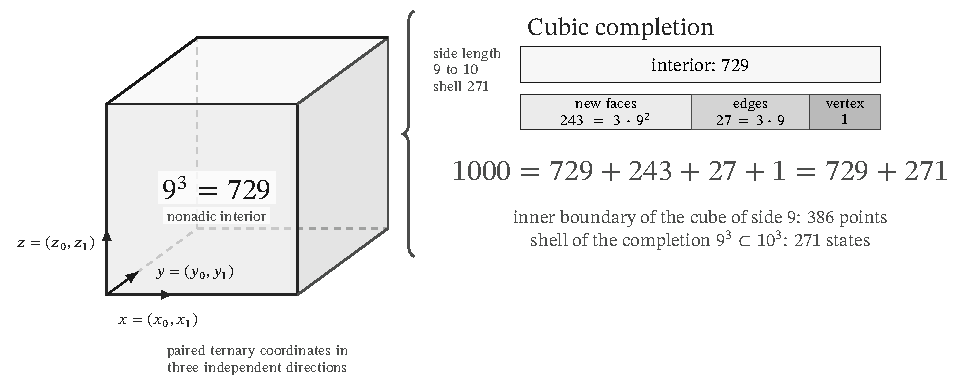
\includegraphics[width=\linewidth]{figures/cubo_emrh.pdf}
\caption{Cubic representation of the expansion from nine to ten classes per coordinate. Strata \(S_1,S_2,S_3\) locate the added incidences on faces, edges, and the apex; their cardinalities form the \(271\)-element shell. The \(386\)-element boundary belongs to the initial cube. This geometric perspective complements the partition in Figure~\ref{fig:revision-emrh}; graphical spacing is schematic.}
\label{fig:completacion-cubo-recuperado}
\end{figure}


\subsubsection{Preservation of unity and dimensional compatibility}

Normalization is not limited to dividing an isolated identity. In dimension
\(d\), the product \(\widehat E^d\) carries the uniform measure
\(\mu_d(\{x\})=10^{-d}\). The coordinate projection
\(p_d:\widehat E^{d+1}\to\widehat E^d\) deletes the final coordinate.

\begin{proposition}[Projective compatibility of the normalized measures]
For every \(d\geq1\),
\[
 (p_d)_*\mu_{d+1}=\mu_d,
 \qquad \mu_d(\widehat E^d)=1.
\]
The mass of the stratum with \(r\) additional coordinates is
\(\binom dr9^{d-r}/10^d\), and the sum of the masses of all strata
is one.
\end{proposition}
\begin{proof}
Every point of \(\widehat E^d\) has ten preimages. Their total mass is
\(10\,10^{-(d+1)}=10^{-d}\). Equality for any subset
is obtained by summing over its points. The stratified formula follows
from the same count as \eqref{eq:revision-estratos}; the binomial
\((9+1)^d\) gives the total normalization.
\end{proof}

In dimension three, removing the apex leaves mass \(999/1000\), and
restoring it adds \(1/1000\). Renormalizing before restoration
would define a different measure: the distinction is operationally relevant.
In particular, preservation of probability mass, preservation of
transport records, and thermodynamic dissipation are assertions concerning
different objects. The proposition proves the first and provides the
compatible support for studying the second; the third requires a
specified dynamical and energetic realization.

The internal geometric boundary likewise remains distinct.
On the Cartesian representative \(\{1,\ldots,9\}^3\), removing
\(\{2,\ldots,8\}^3\) leaves \(386\) points. This boundary belongs to the
initial cube, whereas \(\widehat C\setminus C\) belongs to its
enlargement. The cubic completion, the base-one-thousand positional expansion,
and the exceptional-incidence reading share support data;
their respective maps determine which information from those data is used by
each representation.


\subsection{Cubic incidence and Lorentzian realization}

The cubic completion provides a relation between interior and boundary.
Its geometry can be developed through the incidence of the six faces
with the eight vertices. Label the faces by \((i,\varepsilon)\),
\(i\in\{1,2,3\}\), \(\varepsilon\in\{+1,-1\}\), and the vertices by
\(\nu\in\{+1,-1\}^3\). The incidence matrix is
\[
 M_{(i,\varepsilon),\nu}=\mathbf1_{\{\nu_i=\varepsilon\}}.
\]
Let \(u=(1,\ldots,1)^{\mathsf T}\in\RR^6\), let \(R_F\) denote face
opposition, and let \(P_u=uu^{\mathsf T}/6\), \(P_-=(I-R_F)/2\).

\begin{proposition}[Four-dimensional incidence quotient]
The incidence Gram matrix satisfies
\[
 MM^{\mathsf T}=12P_u+4P_-.
\]
Its eigenvalues \(12,4,0\) have multiplicities \(1,3,2\).
Consequently,
\[
 Q_\square=\RR^6/\ker(MM^{\mathsf T})
 \simeq\RR u\oplus E_-,\qquad E_-=\operatorname{im}P_-.
\]
\end{proposition}
\begin{proof}
A face contains four vertices; two opposite faces have empty intersection,
and two distinct nonopposite faces share two vertices.
The matrix \(12P_u+4P_-\) has precisely those entries.
The uniform space has dimension one; the differences between opposite
faces generate a three-dimensional space orthogonal to the uniform one.
Its complement has dimension two and lies in the kernel.
\end{proof}

The \(1+3\) decomposition arises from incidence. The temporal choice
is specified by the bilinear form
\[
 B_\square([x],[y])=\langle x,(P_--P_u)y\rangle.
\]
It is well defined on the quotient because both projections annihilate the
kernel. In the basis
\[
 t=[u]/\sqrt6,\qquad
 d_i=[e_{i,+}-e_{i,-}]/\sqrt2,
\]
its matrix is \(\operatorname{diag}(-1,1,1,1)\). This makes explicit
the domain, the decomposition, and the sign convention that produce
the Minkowski realization. The positive Gram matrix determines the quotient;
the temporal assignment determines the indefinite form on it.

The operator
\[
 W_\square=\sqrt6P_u+\sqrt2P_-,\qquad
 W_\square e_{i,\varepsilon}=t+\varepsilon d_i
\]
maps the six face labels to null directions, since
\(B_\square(t+\varepsilon d_i,t+\varepsilon d_i)=-1+1=0\).
Direction reversal and face opposition thus acquire a concrete
geometric realization.

\subsubsection{Gluing, reversal, and subdivision}

The cellular realization uses an invertible transport \(U_m(a)\),
which preserves the Lorentzian form, between the fibers at the endpoints of
an oriented dual edge \(a\), a face label
\(\lambda_m(a)\), and an orientation \(\sigma_m(a)\).
With \(\ell_m=\ell_0/9^m\), the gluing map is
\[
 \beta_m(a)=\ell_m\sigma_m(a)
 W_{\square,s(a)}e_{\lambda_m(a)}.
\]
Compatible reversal satisfies
\[
 \beta_m(\bar a)=-U_m(a)\beta_m(a).
\]
Identify the source fibers at two consecutive levels by means of
the specified refinement isometry. If the nine subsegments
\(a_1,\ldots,a_9\), at level \(m+1\), preserve the label
and orientation when transported to that common fiber, then
\begin{equation}
 \beta_m(a)=\sum_{j=1}^9
 U_{m+1}(a_1\cdots a_{j-1})^{-1}\beta_{m+1}(a_j).
 \label{eq:soldadura-refinamiento}
\end{equation}
Each transported term equals \(\ell_m/9\) times the same
null direction, which proves the identity. The compatibility hypothesis
determines which subdivisions realize this refinement.
The equation brings together direction, scale, and transport, instead of reducing
the geometric correspondence to a dimension count.

Once the orientation and Lorentzian form have also been fixed, Hodge duality
on \(\Lambda^2Q_\square^*\) satisfies \(\star^2=-I\).
In dimension four, the sign is \((-1)^{2(4-2)+1}=-1\).
This yields a real complex structure on two-forms and, after
complexification, the eigenspaces with eigenvalues \(+i\) and
\(-i\). The electromagnetic realization will use this domain
after constructing the electronic section and specifying its coupling.

\subsection{Compatibility between modular and positional reductions}

The block-decimal base enters through Euclidean division,
which simultaneously preserves residue and quotient:
\[
 n=1000q+r,\qquad 0\le r<1000.
\]
Since \(1000\equiv1\pmod9\) and \(1000\equiv1\pmod3\),
\[
 n\equiv q+r\pmod9,\qquad n\equiv q+r\pmod3.
\]
Therefore, reduction of a block requires the contribution of the
quotient in order to recover the class of the integer. The numbers \(0\) and
\(1000\) have the same remainder modulo \(1000\), but different classes
modulo \(9\) and modulo \(3\). This is an operational reason to preserve
memory during a change of resolution.

Ternary refinement and determination of a decimal prefix
can be coordinated by means of a single integer residue. If \(N/3^L\)
is a cylinder endpoint and \(D/1000^r\) a decimal endpoint, define
\[
 A=1000^rN-D3^L.
\]
Upon adding six ternary symbols, \(N'=729N+\nu\),
\(L'=L+6\), with \(0\le\nu<729\). If the decimal prefix remains
fixed, then
\[
 A'=729A+\nu1000^r.
\]
If a decimal block \(\delta\) is also incorporated, then
\(D'=1000D+\delta\), \(r'=r+1\), and
\begin{equation}
 A'=729000A+\nu1000^{r+1}-729\delta3^L.
 \label{eq:residuo-dos-bases}
\end{equation}
Both identities are proved by substituting the definitions. Comparison
of endpoints is thus reduced to integer operations that retain the
contribution of each extension. This compatibility is what permits a region
to be refined before its real coordinate is evaluated.

% Incorporated at the end of extension.tex; contains no main section.
% Provenance: RECOVERED_RESULT; sectorial explication of the hypotheses.
% Sources consulted: Holographic Double Projection monograph (editorial source),
% manuscrito/local/01_tesis_recuperada.tex and
% manuscrito/generated/algebra_holonomica.tex, especially §§1--7 and 21.
% Governing definition of number: manuscrito/flattened/main_autosuficiente.tex,
% sections beginning at lines 22137 and 23000 of the 775-page source.
% Its global presentation is not adopted as proof of all TPK arrows.

\subsection{Number as a compatible section and value as a reading}
\label{hist:seccion}

The distinction between state and observation makes it possible to specify which object is
extended as resolution increases. At depth \(n\), let \(X_n\)
be the set of admissible states produced by APP--TRIT--TPK. Their data
include position, sum and product sheets, residues and quotients, regime,
orientation, carry, phase, route, boundary, memory, and survival. These are not
independent coordinates: the arithmetic evaluations and preceding transports
impose their relations. An extension preserves those relations in every
antecedent, even as it adds new steps and new memory data.
This is the meaning of the arithmetic of histories developed self-sufficiently
in this article.

Let \(r_{m,n}:X_m\to X_n\), for \(m\geq n\), be the depth
restrictions, with \(r_{n,n}=\operatorname{id}\) and
\(r_{\ell,n}=r_{m,n}\circ r_{\ell,m}\). Each restriction preserves the
prefix and the information already determined in it.

\begin{definition}[Compatible numerical section]
An HMT number is a compatible history of the system of states:
\begin{equation}
 x=(x_n)_{n\geq0}\in X_\infty:=\varprojlim_n X_n,
 \qquad r_{m,n}(x_m)=x_n.
 \label{hist:limite-inverso}
\end{equation}
A reader is an additional operation on a specified domain of these
histories. A digit is a finite observation; a scalar value is an
evaluation of the reader. The pair formed by the section and its reader constitutes
a read presentation, not a redefinition of the identity of the section.
\end{definition}

On the Archimedean domain \(X_\infty^{\mathrm{Arch}}\), the reader associates
with each prefix a closed cylinder, preserves their nesting, and makes
their diameter tend to zero. It thereby determines
\begin{equation}
 \operatorname{ev}_{\mathbb R}:X_\infty^{\mathrm{Arch}}\longrightarrow
 \mathbb R,\qquad
 \{\operatorname{ev}_{\mathbb R}(x)\}=\bigcap_n I_n(x).
 \label{hist:evaluacion}
\end{equation}
The concrete construction of these cylinders and the determination of their boundaries
are developed in Section~\ref{sec:generacion}. Definition
\eqref{hist:limite-inverso} does not by itself assert that the image of
\eqref{hist:evaluacion} is the entire real line: a coverage assertion
requires its own theorem. Nor does equality of values establish equality of
their histories without an injectivity result. This separation
makes it possible to speak of precision as depth while preserving the distinction
between the arithmetic antecedent and its scalar realization.

\subsection{Composition of histories and memory multiplier}
\label{hist:algebra}

Fix a sector of states at depth \(n\) and a category
\(\mathcal C\) whose arrows are its admissible histories. Composition
is written \(vu=v\circ u\): first \(u\) is traversed and then \(v\).
The elementary steps arise from selection, transport, and the
TPK update. A local tritic fiber can be written
\(\mathbb R[J_x]/(J_x^2+\tau(x)1_x)\), where
\(\tau(x)\in\{+1,0,-1\}\). The regime and orientation belong to the
state being transported; a transition between regimes is not equivalent to
identifying their quadratic algebras.

The following formulation specifies an algebraic sector of that composition.
For each object \(x\), let \(A_x\) be a unital associative real algebra,
which may be noncommutative. For each \(u:x\to y\), let
\(\rho_u:A_x\to A_y\) be a unital homomorphism. Assume a strict action:
\begin{equation}
 \rho_{\operatorname{id}_x}=\operatorname{id}_{A_x},\qquad
 \rho_v\rho_u=\rho_{vu}.
 \label{hist:accion-estricta}
\end{equation}
For each composable pair \(u:x\to y\), \(v:y\to z\), fix an
invertible central multiplier
\(\Omega(v,u)\in Z(A_z)^\times\). Require the normalization
\(\Omega(\operatorname{id}_y,u)=\Omega(u,\operatorname{id}_x)=1_y\)
and, for every composable triple, the identity
\begin{equation}
 \rho_w\bigl(\Omega(v,u)\bigr)\Omega(w,vu)
   =\Omega(w,v)\Omega(wv,u).
 \label{hist:cociclo}
\end{equation}
These are explicit hypotheses on the transports and their coefficients, not a
consequence of calling the dynamics holonomic. When applying this presentation
to a TPK sector, its \(\rho_u\) and \(\Omega(v,u)\) must be identified.
Transitions expressed through bimodules require preservation of that
structure and are not replaced by \eqref{hist:accion-estricta}.

The space of finite sums
\[
 \mathcal H(\mathcal C,A,\rho,\Omega)
   =\bigoplus_{u\in\operatorname{Mor}(\mathcal C)} A_{t(u)}T_u
\]
receives the bilinear product
\begin{equation}
 (aT_v)(bT_u)=a\rho_v(b)\Omega(v,u)T_{vu},
 \label{hist:producto}
\end{equation}
if the arrows are composable, and zero otherwise. Here \(t(u)\)
denotes the terminal state. The sum gathers histories with coefficients; the
product concatenates histories while preserving the record multiplier.

\begin{proposition}[Sectorial associativity with a central multiplier]
Under \eqref{hist:accion-estricta} and \eqref{hist:cociclo}, the product
\eqref{hist:producto} is associative. If the set of objects is finite,
its identity is \(\sum_x1_xT_{\operatorname{id}_x}\).
\end{proposition}
\begin{proof}
For \(u:x\to y\), \(v:y\to z\), \(w:z\to t\), let
\(a\in A_y\), \(b\in A_z\), \(c\in A_t\). The two coefficients
of \(T_{wvu}\) are
\begin{align*}
 ((cT_w)(bT_v))(aT_u):\quad&
 c\rho_w(b)\Omega(w,v)\rho_{wv}(a)\Omega(wv,u),\\
 (cT_w)((bT_v)(aT_u)):\quad&
 c\rho_w(b)\rho_w\rho_v(a)\rho_w(\Omega(v,u))\Omega(w,vu).
\end{align*}
The strict action identifies \(\rho_w\rho_v(a)\) with \(\rho_{wv}(a)\).
Centrality of \(\Omega(w,v)\) permits moving it to the right of
that factor; \eqref{hist:cociclo} then equates the remaining products.
The coefficients \(a,b,c\) are not permuted. If the triple is not composable,
both parenthesizations are zero because of their initial and terminal states.
Bilinearity completes the proof. The local identities and the
normalization of \(\Omega\) verify the stated identity element.
\end{proof}

The calendar carry provides an effective example. In the category
with one object and arrows \(C_9\), take coefficients
\(A=\mathbb R[z,z^{-1}]\), the identity action, and
\[
 \Omega(b,a)=z^{c_0(a,b)},\qquad
 c_0(a,b)=\left\lfloor\frac{a+b}{9}\right\rfloor,
 \quad 0\leq a,b<9.
\]
The two sums of carries of a triple are
\(\lfloor(a+b+c)/9\rfloor\); hence
\eqref{hist:cociclo} holds. The formal variable \(z\) records the circuit without
assigning it a numerical value. Subsequently imposing \(z^{12}=1\) recovers the
dodecaphase register of calendar \eqref{eq:extension108}; retaining
\(z\) without that relation distinguishes successive circuits. The example realizes
the memory of this calendar without identifying it with the entirety of
TPK memory.

\subsection{Dual variance of refinement and preservation of unity}
\label{hist:doble-varianza}

When states are restricted, observables are extended in the opposite direction.
Consider the function algebras, with pointwise product,
\(D_n=\operatorname{Fun}(X_n,\mathbb R)\). Precomposition defines
\begin{equation}
 r_{m,n}^*:D_n\longrightarrow D_m,
 \qquad r_{m,n}^*f=f\circ r_{m,n}.
 \label{hist:precomposicion}
\end{equation}
These are unital morphisms; they are also injective when the corresponding
restrictions are surjective. The direct limit
\(D_{\mathrm{cyl}}=\varinjlim_n(D_n,r_{n+1,n}^*)\) gathers the
finite-depth observations. This algebra is not identified here
with the entire path algebra: extending the transport operators also requires
their compatibilities with refinement.

\begin{lemma}[Unity and naturality of evaluation]
If \(e_x\) is the indicator of \(x\in X_n\), then
\begin{equation}
 r_{m,n}^*e_x=\sum_{y:\,r_{m,n}(y)=x}e_y,
 \qquad r_{m,n}^*1_n=1_m,
 \label{hist:unidad}
\end{equation}
and, for every \(f\in D_n\), \(y\in X_m\),
\[
 \langle r_{m,n}^*f,y\rangle=\langle f,r_{m,n}y\rangle.
\]
Each section \(x\in X_\infty\) determines a well-defined evaluation
\(D_{\mathrm{cyl}}\to\mathbb R\), given by \([f]\mapsto f(x_n)\)
for \(f\in D_n\).
\end{lemma}
\begin{proof}
The fibers of \(r_{m,n}\) form a partition of \(X_m\). Their
indicators are orthogonal and sum to \(1_m\), which proves
\eqref{hist:unidad}. Naturality is the definition of precomposition.
Finally, \((r_{m,n}^*f)(x_m)=f(x_n)\), so two compatible
representatives give the same evaluation in the direct limit.
\end{proof}

The global identity is the constant-one function on all possibilities;
the individual section selects a compatible history. Preserving the
former does not mean immobilizing the latter. Refinement can increase
the number of extensions and the depth of each history while preserving
the identity and all evaluations of its antecedents.

\subsection{Phase return, Weyl representation, and two readings}
\label{hist:puente-lecturas}

Law \eqref{eq:holonomia-memoria} acquires an operator realization
in the bilateral suspension to be constructed in
Section~\ref{sec:generacion}. There \(T\) advances one step,
\(V_9\) observes the nonadic phase, \(W_\delta\) the rotational phase, and
\(D_M\) the memory degree. Writing
\(\widehat\Gamma_9=T^9\) for one circuit in this representation,
the Weyl relations \eqref{eq:weyl-relojes} imply, on vectors
of finite support,
\begin{equation}
 \begin{aligned}
 V_9\widehat\Gamma_9&=\widehat\Gamma_9V_9,\qquad
 W_\delta\widehat\Gamma_9=e^{2\pi i9\delta}
     \widehat\Gamma_9W_\delta,\\
 [D_M,\widehat\Gamma_9]&=\widehat\Gamma_9.
 \end{aligned}
 \label{hist:tres-retornos}
\end{equation}
The first equality follows from \(\zeta_9^9=1\); the second from nine
applications of the covariance of \(W_\delta\); the third expresses
the unit increment of memory. The finite phase returns, while the
irrational rotation and memory distinguish the succeeding state. The
characters and parameter \(\delta\) are realized subsequently from the
numerical construction specified there: they do not retrospectively select
the seeds. This representation describes observables and translations of
the suspension; it does not replace all coordinates or all TPK operators.

The dual reading extends the same distinction between history and observable.
On its Archimedean domain, \eqref{hist:evaluacion} applies; on the
enriched incidence domain, the maps \(Q_n\) of
Section~\ref{exc:doble-lectura} preserve the words and boundary
frames. The equality proved there,
\(r_{n,m}Q_n=Q_mp_{n,m}\), determines its extension \(Q_\infty\).
On the common domain of both readings,
\(\operatorname{ev}_{\mathbb R}(x)\) and \(Q_\infty(x)\) may be considered jointly: the
first retains the value; the second, the transported incidence preserved by its
codomain. The section precedes both. This articulation makes it possible
to pass from the arithmetic of histories to constants and the exceptional
reading without turning their realizations into new initial data.

